\date{3/8/2015}
\title{\so\\Introdução}

\frame{\maketitle}

\section{Introdução}

\begin{frame}{Sistemas de computação}

\usetikzlibrary{shapes}%add to preambule if the main file does not compile

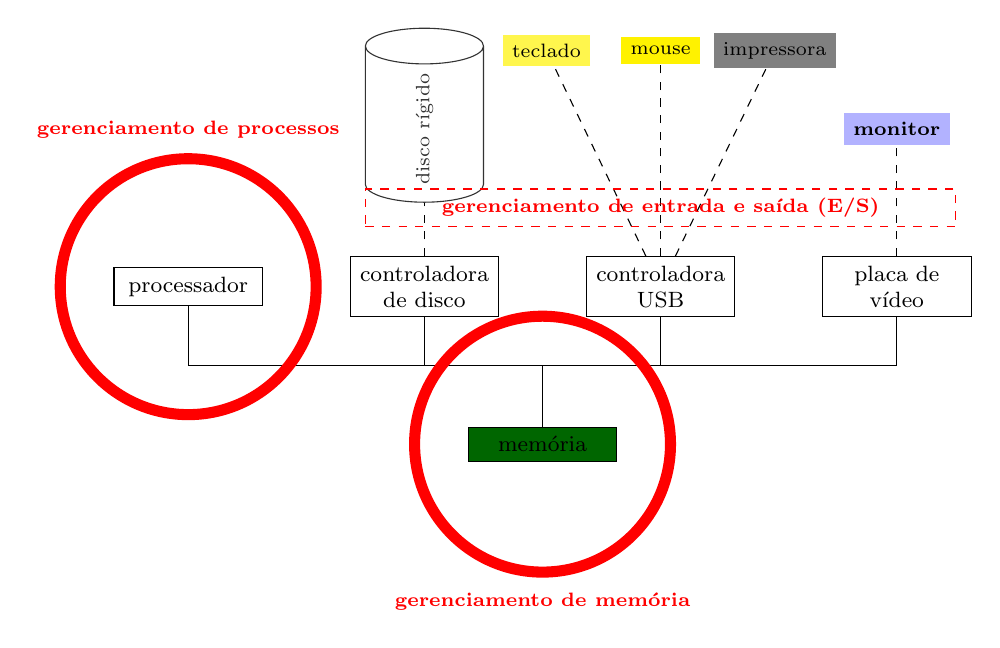
\begin{tikzpicture}[control/.style={text width=1.65cm,align=center,font=\footnotesize,draw},
    every path/.style={draw},device/.style={fill=yellow,font=\scriptsize,minimum width=1cm},
    device connection/.style={dashed},
    disk/.style={black!80,font=\scriptsize,cylinder,minimum width=1.5cm,rotate=90,draw},
    os module/.style={minimum size=3.25cm,circle,red,line width=4,text width=2cm,draw},
    module label/.style={red,font=\bf\scriptsize}]

    \def\dx{3cm}
    \def\dy{2cm}
    
    \node[control] (proc) at (0,0) {processador};
    \node[control] (disk controller) at (\dx,0) {controladora de disco};
    \node[control] (usb controller) at (2*\dx,0) {controladora USB};
    \node[control] (video card) at (3*\dx,0) {placa de vídeo};
    \node[control,fill=green!40!black] (mem) at (1.5*\dx,-\dy) {memória};

    \path (proc) -- +(0,-0.5*\dy) -- +(3*\dx,-0.5*\dy) -- +(video card);
    \path (\dx,-0.5*\dy) -- +(disk controller);
    \path (2*\dx,-0.5*\dy) -- +(usb controller);
    \path (1.5*\dx,-0.5*\dy) -- +(mem);

    \node[disk] (hd) at (\dx,\dy) {disco rígido};
    \path[device connection] (disk controller) -- (hd);

    \node[device] (mouse) [above of=usb controller,yshift=\dy] {mouse};
    \node[device,fill=gray] (printer) [right of=mouse,xshift=.15*\dx] {impressora};
    \node[device,fill=yellow!70] (keyboard) [left of=mouse,xshift=-.15*\dx] {teclado};
    \path[device connection] (usb controller) -- (mouse);
    \path[device connection] (usb controller) -- (printer);
    \path[device connection] (usb controller) -- (keyboard);

    \node[device,fill=blue!30] (monitor) [above of=video card,yshift=.5*\dy] {\bf monitor};
    \path[device connection] (video card) -- (monitor);

    \node<2>[os module] (proc module) at (proc) {};
    \node<2>[module label] [above of=proc module,yshift=.5*\dy] {gerenciamento de processos};

    \node<3>[os module] (mem module) at (mem) {};
    \node<3>[module label] [below of=mem module,yshift=-.5*\dy] {gerenciamento de memória};

    \node<4>[module label,minimum width=7.5cm,dashed,draw] [above of=usb controller] {gerenciamento de entrada e saída (E/S)};
  \end{tikzpicture}


\end{frame}

\begin{frame}{Divisão do curso}
  O curso será dividido em $3$ tópicos principais envolvendo
  Gerenciamento de:
  \begin{enumerate}
  \item Processos;
  \item Memória;
  \item Entrada e saída (E/S).
  \end{enumerate}

\end{frame}


\begin{frame}{Complexidade dos \so{}: Microsoft Windows}
\scriptsize
  \begin{tabular}[f]{|c|l|c|c|c|} \hline
    \tiny  Data  &	 Produto &
     \tiny Tam. Equipe  &	\tiny Tam. Equipe  &
     \tiny Linhas de  \\
     \tiny Lançamento &	  &
     \tiny Desenvolvimento &	 \tiny  Teste &
     \tiny Código  (milhões) \\ \hline\hline
    Jul/93 &	NT 1.0 \tiny (release 3.1) &	200 &	140 &	4-5  \\ \hline
    Set/94 &	NT 2.0 \tiny (release 3.5) &	300 &	230 &	7-8  \\ \hline
    Mai/95 &	NT 3.0 \tiny (release 3.51) &	450 &	325 &	9-10  \\ \hline
    Jul/96 &	NT 4.0 \tiny (release 4.0) &	800 &	700 &	11-12 \\ \hline
    Dez/99 &	NT 5.0 \tiny (Windows 2000) &	1.400 &	1.700 &	29+  \\ \hline
    Out/01 &	NT 5.1 \tiny (Windows XP) &	1.800 &	2.200 &	40  \\ \hline
    Abr/03 &	NT 5.2 \tiny (Windows Server 2003) &	2.000 &	2.400 &	50  \\ \hline
  \end{tabular}
  {\tiny Fonte:
    \href{http://www.amazon.com/exec/obidos/ASIN/0321332059/thinkinginnet-20}{``The
      Build Master''. Vicent Maraia, Addison-Wesley, 2005.} }
\end{frame}

%%%%%%%% kernel source graphics
\section{Complexidade dos SOs}

\def\datasource{
  \vspace{-.35cm}
   \color{black!85}{\tiny Fonte: \href{http://www.linuxfoundation.org/}{Linux Foundation}, 
     \url{http://go.linuxfoundation.org/who-writes-linux-2012}}
 }

\begin{frame}{Complexidade dos \so{}: Kernel do Linux}
\framesubtitle<1>{Linhas de código}
\framesubtitle<2>{Quantidade de arquivos}
\begin{center}
\def\graphicone{0}
% Preamble: \pgfplotsset{width=11cm,compat=1.5.1}
\vspace{-.5cm}
\begin{tikzpicture}
  \node<1>[red,rotate=90]  at (-1,3) {linhas de código};
  \node<2>[green!40!black,rotate=90]  at (-1,3) {quantidade de arquivos};
  \begin{axis}[
    grid=major,
    xticklabels={2.6.11,2.6.12, 2.6.13,%
      2.6.14,2.6.15,2.6.16,2.6.17,2.6.18,2.6.19,%
      2.6.20,2.6.21,2.6.22,2.6.23,2.6.24,2.6.25,%
      2.6.26,2.6.27,2.6.28,2.6.29,2.6.30,2.6.31,%
      2.6.32,2.6.33,2.6.34,2.6.35,2.6.36,2.6.37,%
      2.6.38,2.6.39,3.0,3.1,3.2},%
    xtick={1,...,32},
    xticklabel style={rotate=90,anchor=east,text height=2ex,font=\tiny},
    xlabel style={yshift=-.25cm,font=\footnotesize},
    xlabel={versão do kernel},
    ]
\only<1>{
    \addplot[color=red,mark=x] coordinates {
      (1,6624076) (2,6777860) (3,6988800)
      (4,7143233) (5,7290070) (6,7480062)
      (7,7588014) (8,7752846) (9,7976221)
      (10,8102533) (11,8246517) (12,8499410)
      (13,8566606) (14,8859683) (15,9232592)
      (16,9411841) (17,9630074) (18,10118757)
      (19,10934554) (20,11560971) (21,11970124)
      (22,12532677) (23,12912684) (24,13243582)
      (25,13468253) (26,13422037) (27,13919579)
      (28,14211814) (29,14537764) (30,14651135)
      (31,14776002) (32,15004006)
      
      };
}
\only<2>{
  \addplot[color=green!40!black,mark=o] coordinates {(1,17090) (2,17360) (3,18090)
    (4,18434) (5,18811) (6,19251)
    (7,19553) (8,20208) (9,20936)
    (10,21280) (11,21614) (12,22411)
    (13,22530) (14,23062) (15,23813)
    (16,24273) (17,24356) (18,25276)
    (19,26702) (20,27911) (21,29143)
    (22,30504) (23,31584) (24,32316)
    (25,33335) (26,34317) (27,36189)
    (28,36868) (29,36713) (30,36788)
    (31,37095) (32,37626)};
}

\end{axis}
\end{tikzpicture} 
\end{center}
\datasource
\end{frame}

%%%%%%%%%%%%%%%%%%%%%%%%%%%%%%%%
%% Linux report 2015
\def\source{{\scriptsize Fonte: \href{http://www.linuxfoundation.org/publications/linux-foundation/who-writes-linux-2015}{``Who Writes Linux 2015''}}}

\begin{frame}{Complexidade dos \so{}: Kernel do Linux}{Relatório de 2015}

  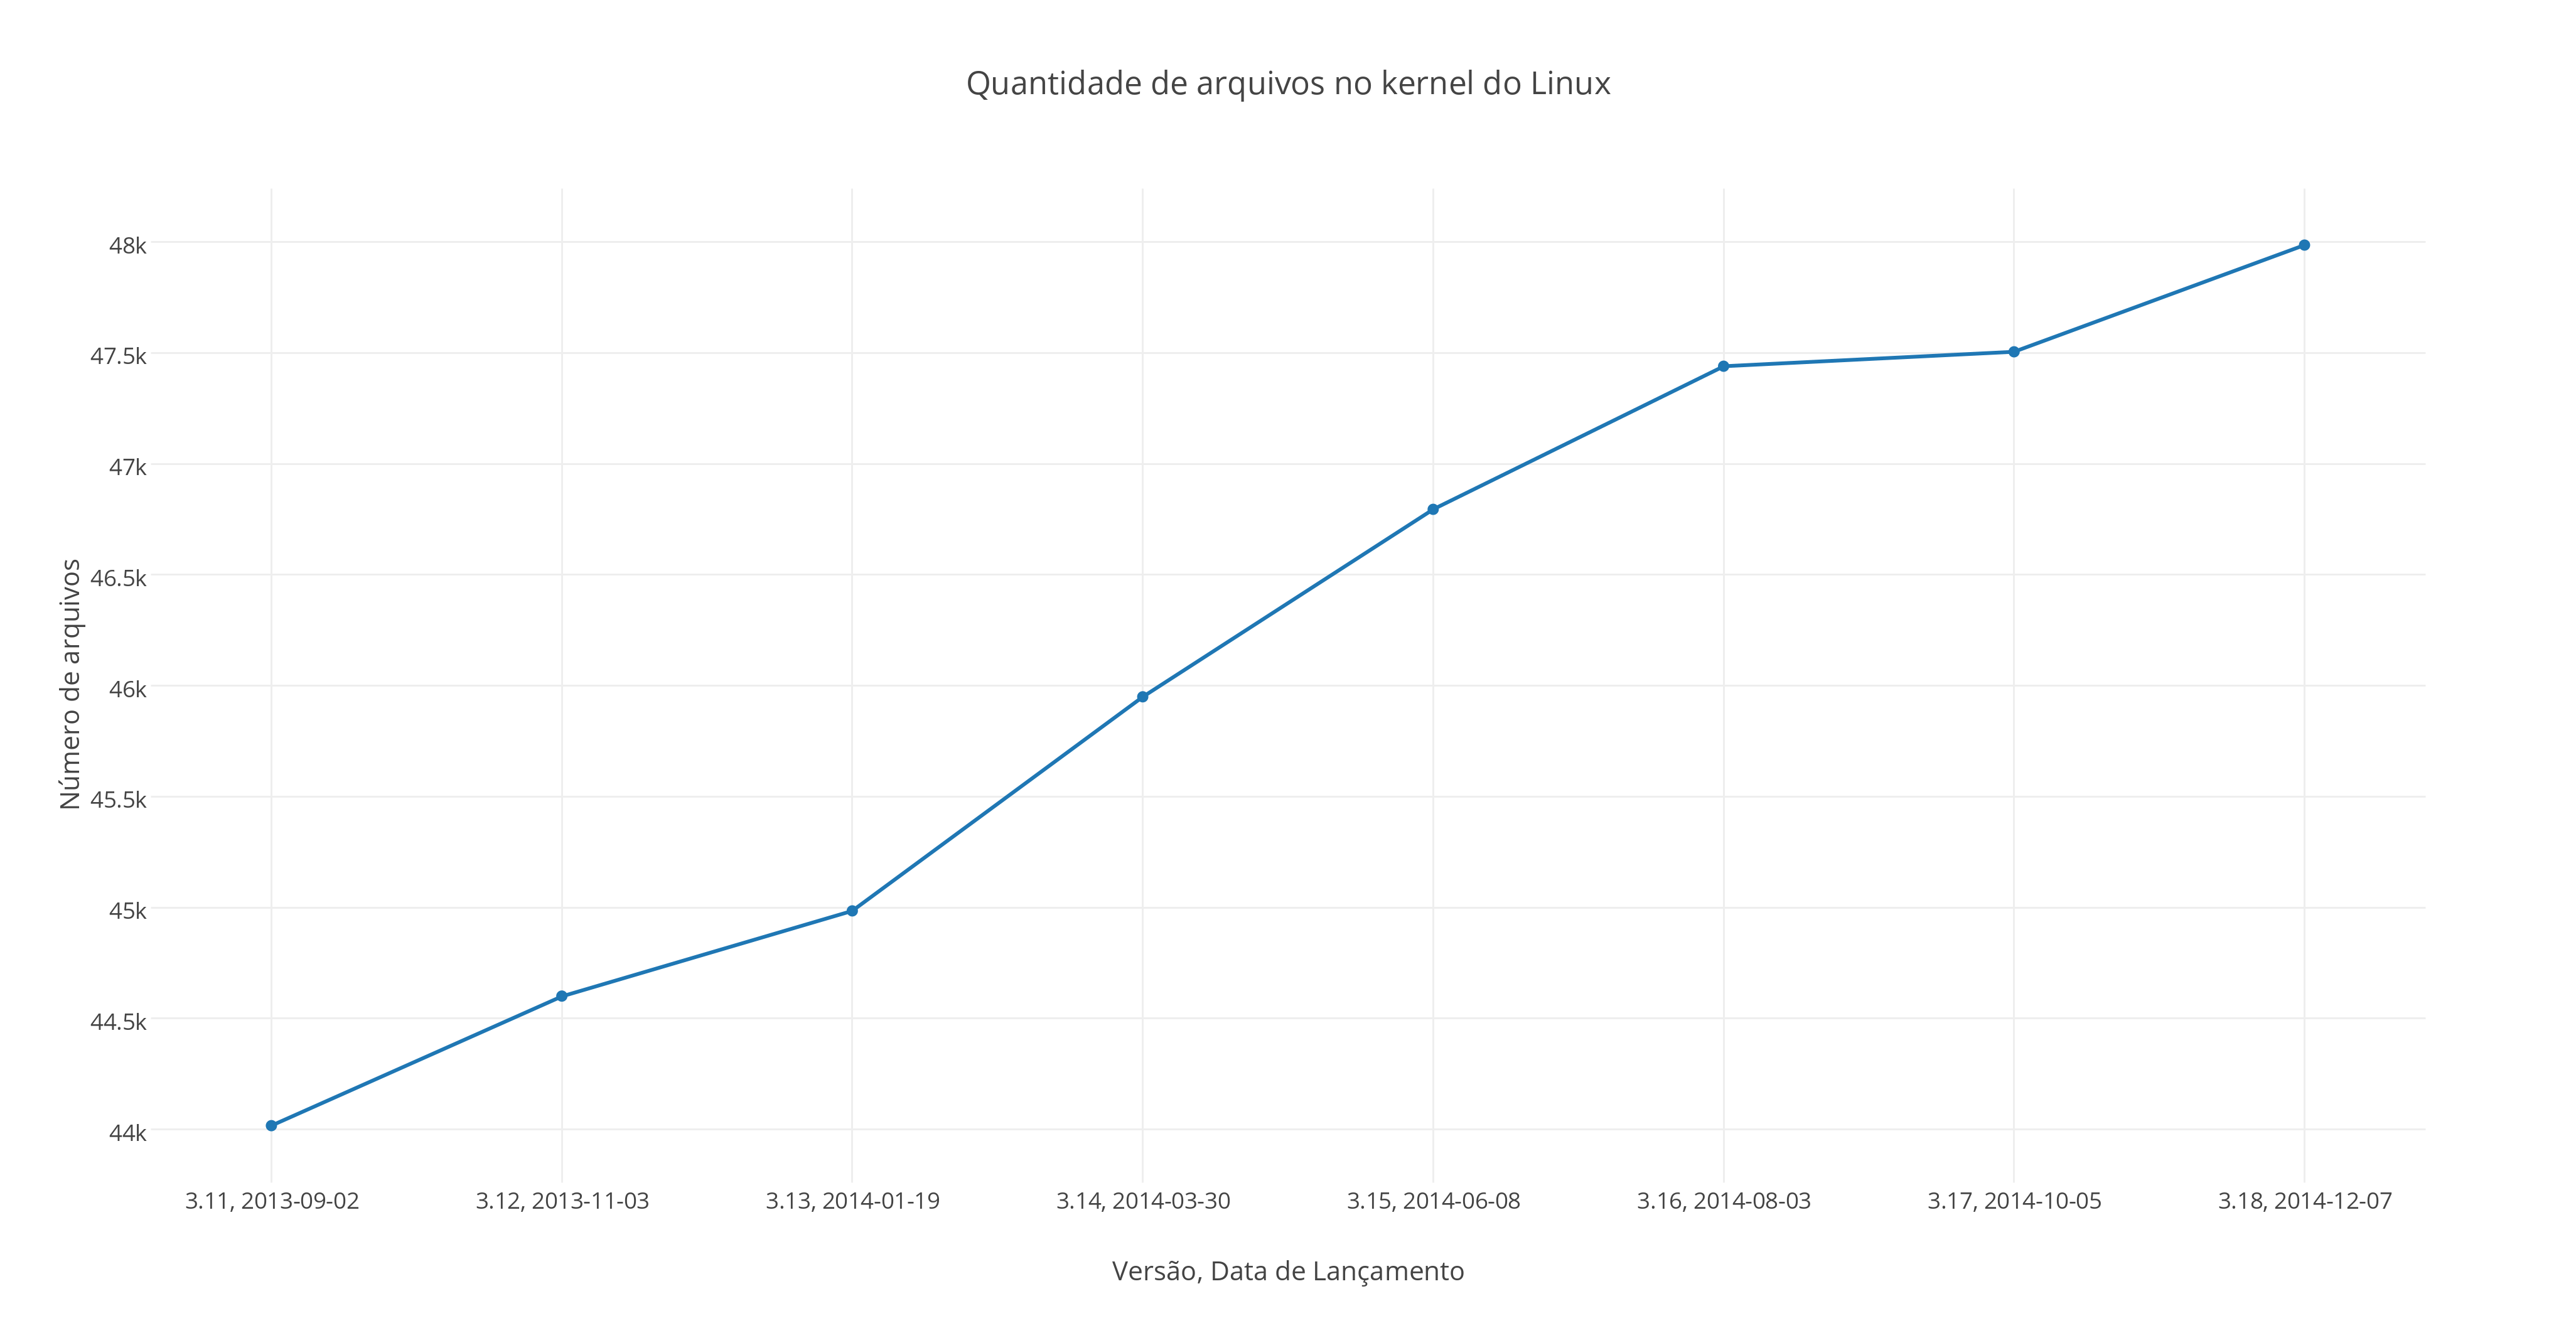
\includegraphics[scale=.35]{img/linux-files-2015.png}

  \source
\end{frame}

\begin{frame}{Complexidade dos \so{}: Kernel do Linux}{Relatório de 2015}
  
  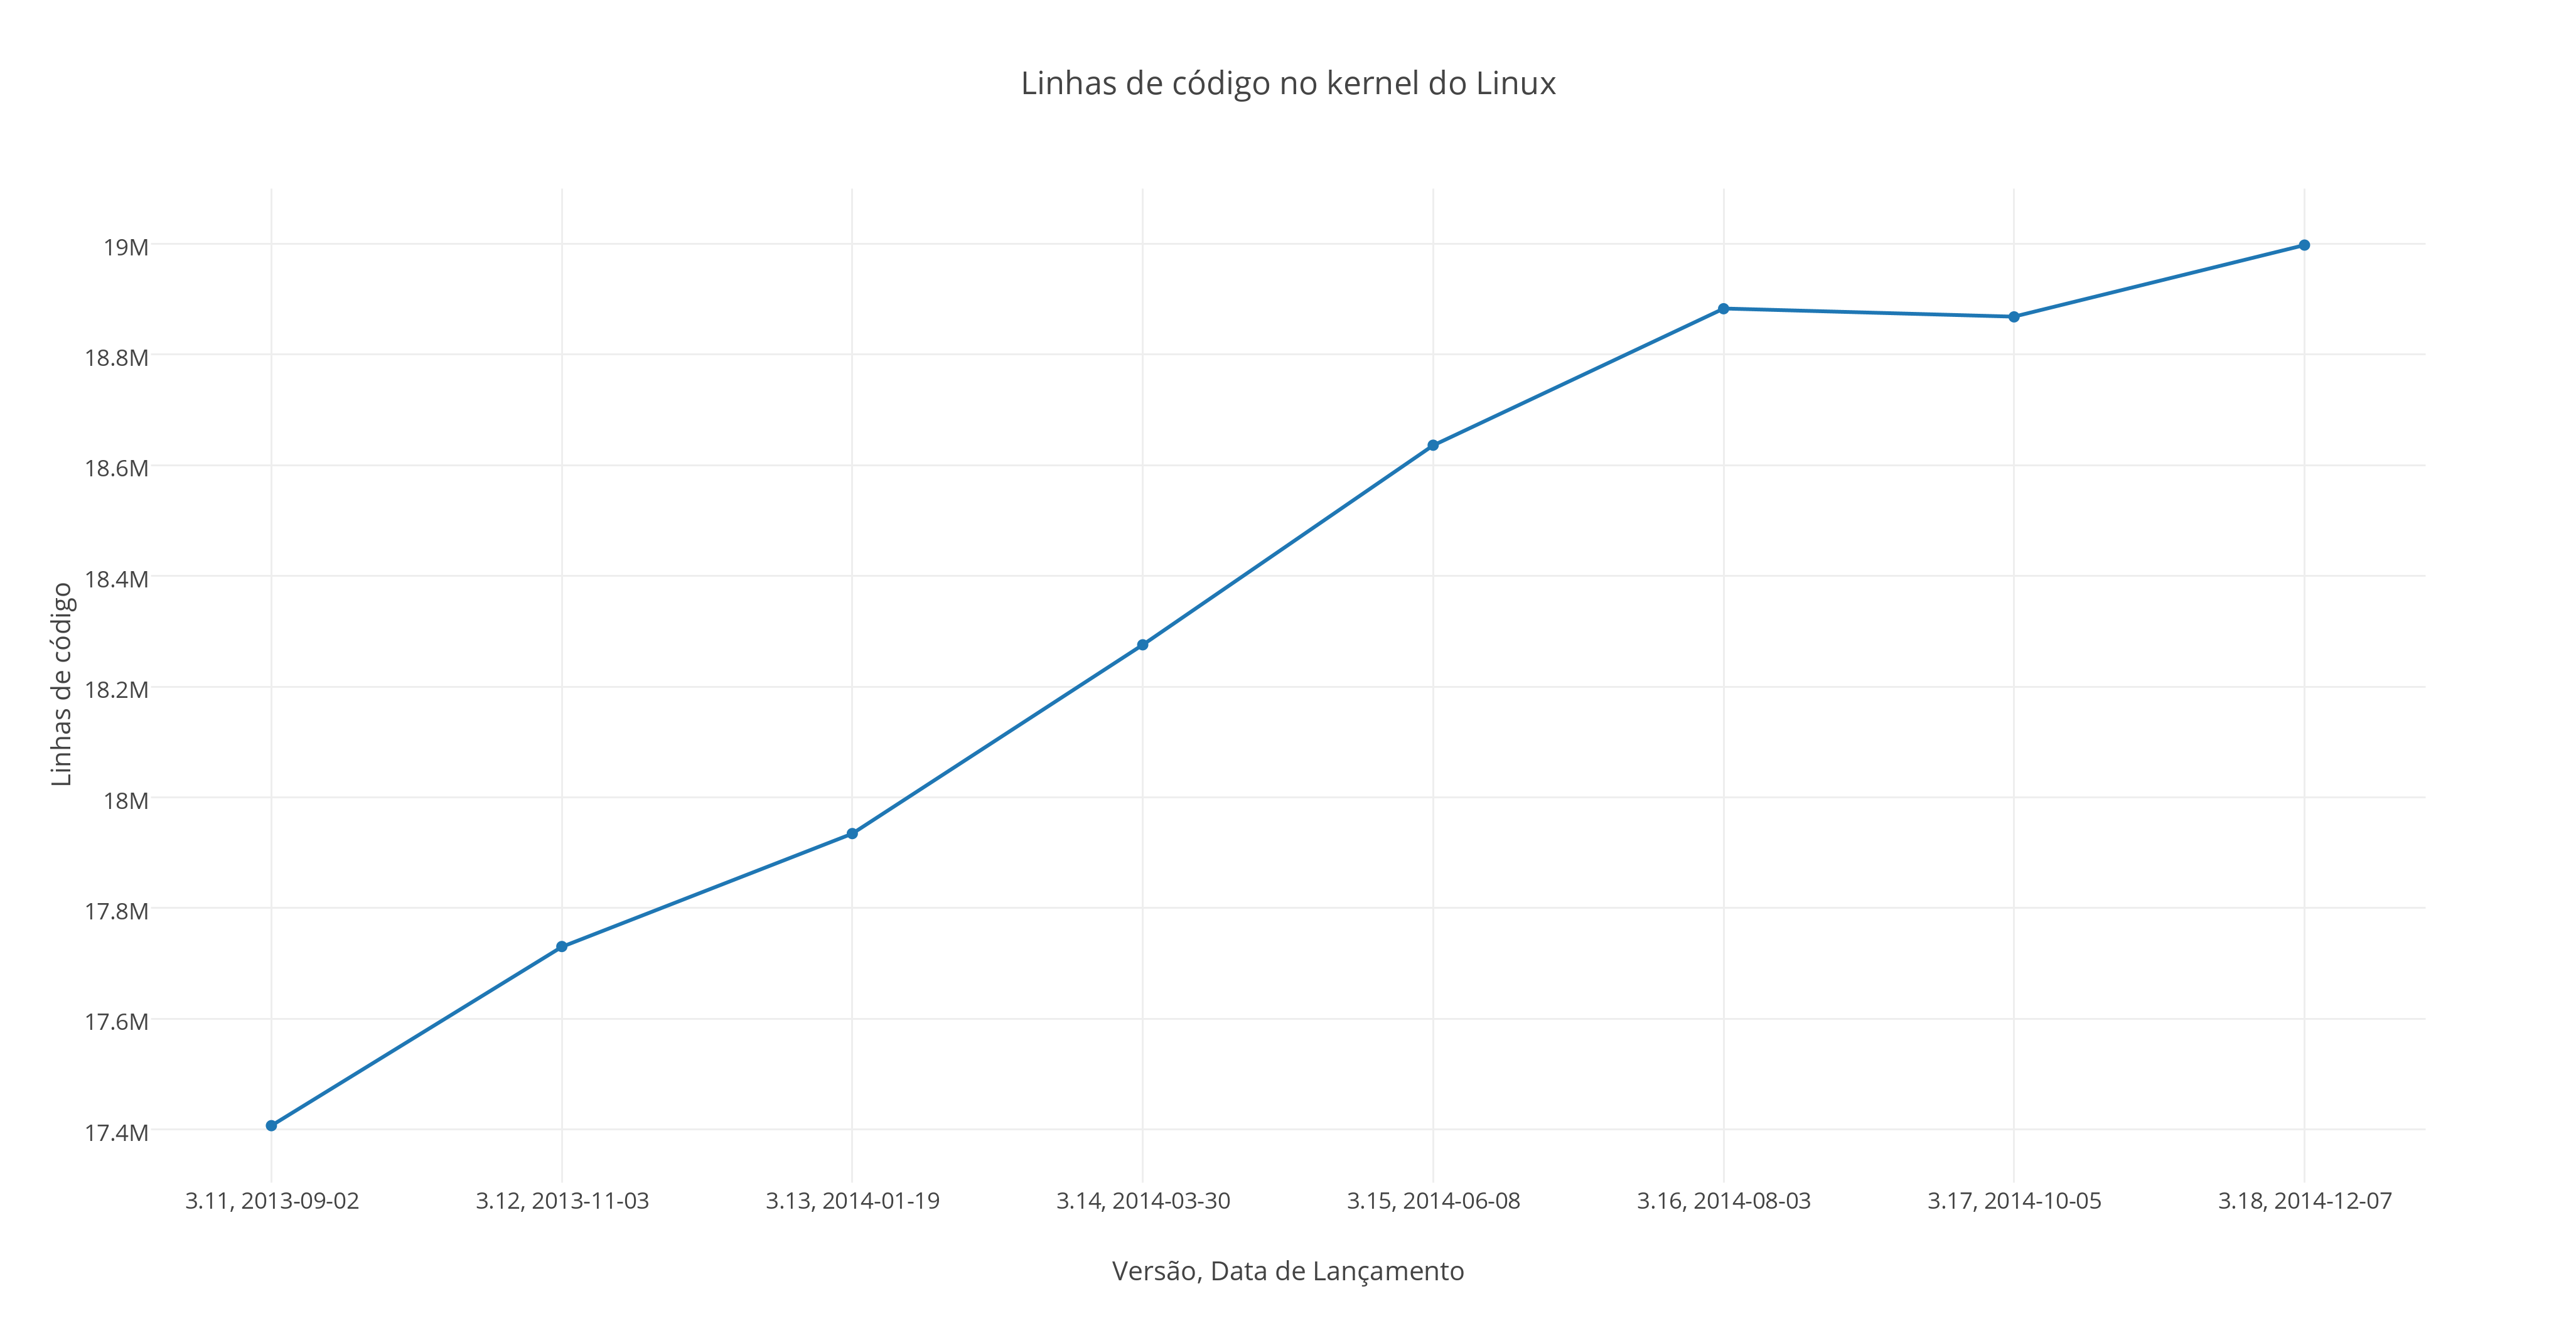
\includegraphics[scale=.35]{img/linux-code-2015.png}

  \source
\end{frame}

\def\sectiontitle{Serviços}
\section{\sectiontitle}

\begin{frame}{\sectiontitle}
  \begin{itemize}
  \item Interface com o usuário
    \begin{itemize}
    \item Linha de comando;
    \item Lote ({\em batch});
    \item Gráfica.
    \end{itemize}
  \item Execução de programa
  \item Operação de Entrada e Saída (E/S)
  \item Manipulação de Sistema de Arquivos
  \item Comunicação
  \item Detecção de erros
\end{itemize}
  
\end{frame}

\def\sectiontitle{Arquitetura dos SOs}

\section{\sectiontitle}

\begin{frame}{\sectiontitle}
  \begin{itemize}
  \item Monolítico;
  \item Micronúcleo.
  \end{itemize}
\end{frame}

\colorlet{kernel color}{black!80}
\colorlet{user color}{blue!40!black}

\begin{frame}{Projeto de núcleo ({\em kernel}) monolítico}
\def\dx{3cm}
\def\dy{2cm}
\vspace{-.75cm}
  \begin{center}
    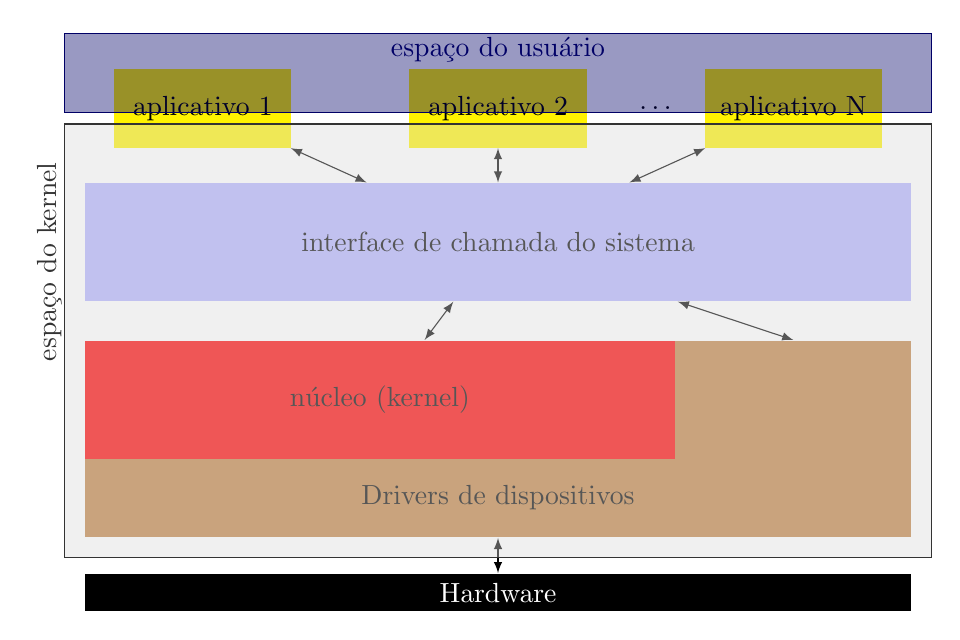
\begin{tikzpicture}[application/.style={fill=yellow,minimum height=.5*\dy,minimum width=.75*\dx}]
      \node[color=white,fill=black,minimum width=3.5*\dx] (hardware) {Hardware};
      \node<2->[fill=brown,minimum height=.5*\dy,minimum width=3.5*\dx] (device driver) [above of=hardware,yshift=.1*\dy] {Drivers de dispositivos};
      \node<2->[fill=brown,minimum height=1*\dy,minimum width=\dx] (top device driver) [above of=device driver,xshift=1.25*\dx] {};
      \node<3->[fill=red,minimum height=.75*\dy,minimum width=2.5*\dx] (kernel) [above of=device driver,xshift=-.5*\dx,yshift=.125*\dy] {núcleo (kernel)};
      \node<4->[fill=blue!30,minimum height=.75*\dy,minimum width=3.5*\dx] (system call) 
      [above of=kernel,xshift=.5*\dx,yshift=.5*\dy] {interface de chamada do sistema};

      \node<5->[application] (app2) [above of=system call, yshift=.35*\dy] {aplicativo 2};
      \node<5->[application] (app1) [left of=app2,xshift=-2.75cm] {aplicativo 1};
      \node<5->[application] (appn) [right of=app2,xshift=2.75cm] {aplicativo N};
      \node<5->[right of=app2,xshift=1cm] {$\dots$};

      \draw<2->[<->,>=latex] (device driver) -- (hardware);
      \draw<4->[<->,>=latex] (kernel) -- (system call);
      \draw<4->[<->,>=latex] (top device driver.north) -- (system call);
      \draw<5->[<->,>=latex] (app1) -- (system call);
      \draw<5->[<->,>=latex] (app2) -- (system call);
      \draw<5->[<->,>=latex] (appn) -- (system call);


      \node<6->[minimum width=11cm,minimum height=5.5cm,anchor=south,fill opacity=.4,fill=gray!30,draw=kernel color] (kernel space) 
      [above of=hardware,yshift=1.1*\dy] {};
      \node<6->[color=kernel color,rotate=90] [right of=kernel space,yshift=2.85*\dy] {espaço do kernel};

      \node<7->[minimum width=11cm,minimum height=1cm,anchor=south,fill opacity=.4,fill=user color,draw=user color] (user space) 
      [above of=kernel space,yshift=1.2*\dy] {};
      \node<7->[color=user color] [above of=user space,yshift=-.35*\dy] {espaço do usuário};


    \end{tikzpicture}
%  \includegraphics[scale=0.49]{img/intro_monolithic.pdf}
\end{center}
\end{frame}

\begin{frame}{Projeto monolítico}{Características}
  \begin{itemize}
  \item Simplicidade: todo o código reside no mesmo espaço de
    endereços de memória compartilhada, evitando o mecanismo de
    comunicação entre processos, que podem ser complexos e prejudicar
    o desempenho do sistema;
  \item Intolerante a falhas: se houver qualquer falha nos {\em
      drivers} ou subsistemas do núcleo, todo o sistema entra em
    colapso ({\em kernel panic}), interrompendo o funcionamento.
  \end{itemize}
\end{frame}

\begin{frame}{Projeto baseado em micronúcleo {\em microkernel}}
\def\dx{3cm}
\def\dy{2cm}

  \vspace{-.5cm}
  \begin{center}
    \colorlet{aplicativo}{blue}
    \colorlet{servidor de}{yellow}
    \colorlet{driver de}{brown}
    \def\slabel{}
    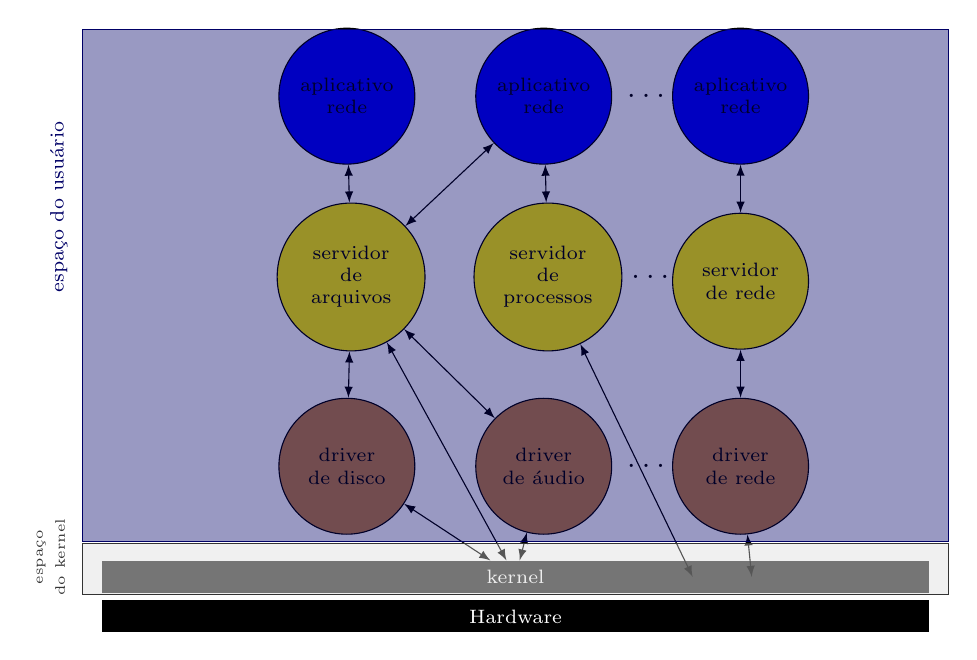
\begin{tikzpicture}[every node/.style={font=\scriptsize,anchor=south west,align=center},
      server/.style={minimum size=1.5cm,circle,draw},
      every path/.style={<->,>=latex,draw}]

      \node<1->[color=white,fill=black,minimum width=3.5*\dx] at (0,0.85cm) (hardware) {Hardware};
      \node<2->[color=white,fill=kernel color,minimum width=3.5*\dx] at (0,1.35cm) (kernel) {kernel};
      
      \foreach \y/\ly/\slide in {1/driver de/3,2/servidor de/4,3/aplicativo/5} {
        \foreach \x in {1,2,3} {
          \ifnum\y=1
          \ifnum\x=1\def\slabel{disco}\fi
          \ifnum\x=2\def\slabel{áudio}\fi
          \ifnum\x=3\def\slabel{rede}\fi
          \fi
          \ifnum\y=2
          \ifnum\x=1\def\slabel{arquivos}\fi
          \ifnum\x=2\def\slabel{processos}\fi
          \ifnum\x=3\def\slabel{rede}\fi
          \fi
          \ifnum\x=3
          \node<\slide-> [right of=s2\y,xshift=.3cm] {\large $\dots$};
          \fi
          
          \node<\slide->[server,fill=\ly,text width=1.35cm] (s\x\y) at (2.5*\x cm,2.35*\y cm) {\ly\ \slabel};
       }
     }
     \path<3-> (kernel) -- (s11);
     \path<3-> (kernel) -- (s21);
     \path<3-> (kernel)+(3cm,0) -- (s31);
     \path<5-> (s11) -- (s12);
     \path<5-> (s12) -- (s13);
     \path<4-> (kernel) -- (s12);
     \path<4-> (kernel)+(2.25cm,0) -- (s22);
     % net
     \path<6-> (s31) -- (s32);
     \path<6-> (s32) -- (s33);
     %audio
     \path<6-> (s21) -- (s12);
     % 
     \path<5-> (s22) -- (s23);
     \path<5-> (s12) -- (s23);

     
     \node<6->[minimum width=11cm,minimum height=.65cm,anchor=south,fill opacity=.4,fill=gray!30,draw=kernel color] (kernel space) 
     [above of=hardware,yshift=-.4cm] {};
     \node<6->[color=kernel color,rotate=90,text width=1.25cm] [right of=kernel,yshift=2.95*\dy,xshift=-.75cm] {\tiny espaço do kernel};

     \node<7->[minimum width=11cm,minimum height=6.5cm,anchor=south,fill opacity=.4,fill=user color,draw=user color] (user space) 
     [above of=kernel space,yshift=1.3*\dy] {};
     \node<7->[color=user color] [above of=user space,rotate=90,yshift=2.9*\dy] {espaço do usuário};


    \end{tikzpicture}
  %\includegraphics[scale=0.45]{img/intro_microkernel.pdf}
\end{center}
\end{frame}

\begin{frame}{Projeto baseado em micronúcleo}{Características}
  \begin{itemize}
    \item Comunicação: troca de mensagens;
    \item Facilidade de extensão: cada serviço pode ser modificado sem
      afetar os outros serviços ou o \so{};
    \item Confiabilidade e segurança: Se algum serviço falhar o \so{}
      permanecerá intocável, pois o serviço é executado no espaço do
      usuário e não afeta o sistema.
  \end{itemize}
\end{frame}

\begin{frame}{Projeto híbrido}
  O projeto híbrido de sistema operacional é uma combinação dos
  projetos monolítico e baseado em micronúcleo, executando alguns
  serviços no espaço do kernel, tais como escalonamento do processador
  e comunicação entre processos, por exemplo, com o objetivo de reduzir a
  sobrecarga causada pela passagem de mensagens destes serviços ao
  microkernel.
\end{frame}

\begin{frame}{Alguns exemplos}
  
  \begin{itemize}
  \item Monolítico: \href{http://www.linux.org/}{Linux} (\href{http://www.android.com/}{Android}),
    \href{http://www.freebsd.org/}{FreeBDS},
    \href{http://www.openbsd.org/}{OpenBSD},
    \href{http://www.netbsd.org/}{NetBSD}, 
    \href{http://www.oracle.com/solaris}{Solaris};
  \item Micronúcleo:
    \href{http://www.gnu.org/software/hurd/hurd.html}{GNU Hurd},
    \href{http://os.inf.tu-dresden.de/L4/}{L4}, 
    \href{http://www.minix3.org/}{Minix},
    \href{http://www.qnx.com/}{QNX};
  \item Híbrido: \href{http://www.apple.com/macosx/}{Mac OS X},
    \href{http://www.microsoft.com/windows/default.aspx}{Microsoft Windows NT/2000/XP/Vista/7 e Server 2003/2008}.
  \end{itemize}
\end{frame}


